\begin{figure}[h!]
  \centering   
    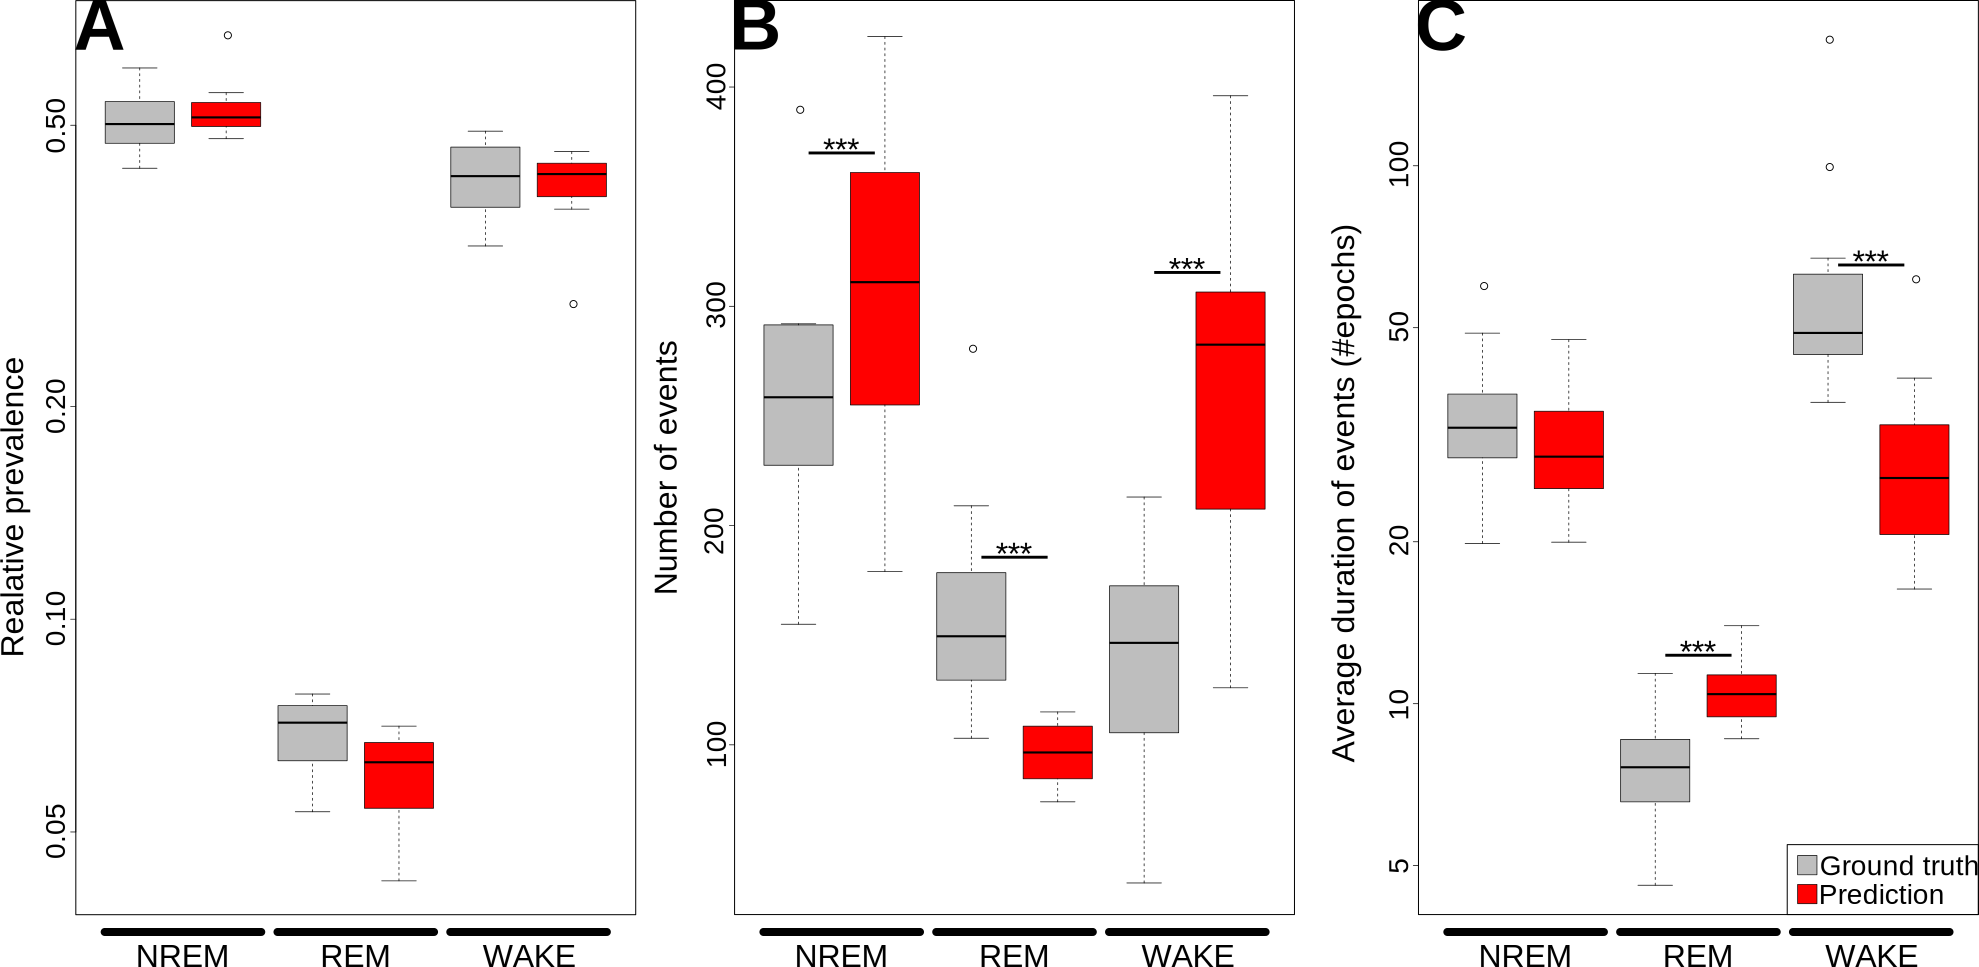
\includegraphics[width=1.0\textwidth]{figures/struct_assess.pdf}
  \caption{\ctit{Structural differences.}
  Three metrics describing structure of sleep were computed for both ground truth (grey) and predicted (red) time series.
  \textbf{A}, No significant difference in state prevalence was found.
  \textbf{B}, The number of events was significantly over-estimated by the classifier
   for wake state and under-estimated for \gls{rem} state ($p-value < 10^{-15}$ for both).
  \textbf{C}, The average duration of wake and \gls{rem} episodes
  were under-estimated ($p-value < 10^{-2}$) and marginally over-estimated ($p-value = 0.057$), respectively.
  Log scale was used for the response variables in A and C. 
  $n = 12$ per combination of factors.
  Statistical methods are detailed in the Material and Methods section.
  Significance levels: $^{***}$, $p-value < 10^{-3}$;  $^{**}$, $p-value < 10^{-2}$.
  \label{fig:struct_assess}
  }
\end{figure}
